%%%%%%%%%%%%%%%%%%%%%%% file template.tex %%%%%%%%%%%%%%%%%%%%%%%%%
%
% This is a general template file for the LaTeX package SVJour3
% for Springer journals.          Springer Heidelberg 2014/09/25
%
% Copy it to a new file with a new name and use it as the basis
% for your article. Delete % signs as needed.
%
% This template includes a few options for different layouts and
% content for various journals. Please consult a previous issue of
% your journal as needed.
%
%%%%%%%%%%%%%%%%%%%%%%%%%%%%%%%%%%%%%%%%%%%%%%%%%%%%%%%%%%%%%%%%%%%
\RequirePackage{fix-cm}
\documentclass[referee]{svjour3}
\newcommand{\remarkpha}[1]{{ \bf PHA:  [ \footnotesize #1 ]}}

\smartqed  % flush right qed marks, e.g. at end of proof
%
%\usepackage{setspace}
%\onehalfspacing
\usepackage{amsmath}
\usepackage{graphicx}
\usepackage{lineno}
\usepackage{natbib}
\linenumbers
%
% \usepackage{mathptmx}      % use Times fonts if available on your TeX system
%
% insert here the call for the packages your document requires
%\usepackage{latexsym}
% etc.
%
% please place your own definitions here and don't use \def but
% \newcommand{}{}
%
% Insert the name of "your journal" with
% \journalname{myjournal}

%
\newcommand*\patchAmsMathEnvironmentForLineno[1]{%
\expandafter\let\csname old#1\expandafter\endcsname\csname #1\endcsname
\expandafter\let\csname oldend#1\expandafter\endcsname\csname end#1\endcsname
\renewenvironment{#1}%
{\linenomath\csname old#1\endcsname}%
{\csname oldend#1\endcsname\endlinenomath}}% 
\newcommand*\patchBothAmsMathEnvironmentsForLineno[1]{%
\patchAmsMathEnvironmentForLineno{#1}%
\patchAmsMathEnvironmentForLineno{#1*}}%
\usepackage{floatpag,mwe}
\usepackage[table]{xcolor}
\usepackage{subfig}
\usepackage{multicol}
\usepackage{afterpage}
\usepackage{color}
\definecolor{greytext}{gray}{0.5}
\definecolor{offyellow}{cmyk}{0, 0, 1, .2}
\usepackage{pifont}
\AtBeginDocument{%
\patchBothAmsMathEnvironmentsForLineno{equation}%
\patchBothAmsMathEnvironmentsForLineno{align}%
\patchBothAmsMathEnvironmentsForLineno{flalign}%
\patchBothAmsMathEnvironmentsForLineno{alignat}%
\patchBothAmsMathEnvironmentsForLineno{gather}%
\patchBothAmsMathEnvironmentsForLineno{multline}%
}

\begin{document}

\graphicspath{{./figures/}}


\title{The effects of stability on idealized convective boundary layer entrainment%\thanks{Grants or other notes
%about the article that should go on the front page should be
%placed here. General acknowledgments should be placed at the end of the article.}
}

\titlerunning{The effects of stability}        % if too long for running head

\author{N.~A.~Chaparro \and P.~H.~Austin \and D.~G.~Steyn
         %etc.
}

%\authorrunning{Short form of author list} % if too long for running head

\institute{ P.~H.~Austin \at
              Department of Earth, Ocean, and Atmospheric Sciences, 
              The University of British Columbia, 
	      Room 2020, Earth Science Building,
              2207 Main Mall,
              Vancouver, BC, 
              V6T 1Z4 \\
              Tel.: +\\
              Fax: +\\
              \email{@eos.ubc.ca}           %  \\
%             \emph{Present address:} of F. Author  %  if needed
           %\and
           %S. Author \at
           %   second address
}

\date{Received: DD Month YEAR / Accepted: DD Month YEAR}
% The correct dates will be entered by the editor


\maketitle

\begin{abstract}

Large eddy simulations (LES) are used to  model a dry, shear-free, idealized convective boundary layer in the absence of large scale winds.  Ten member ensembles are calculated for a range of convective  Richardson numbers yielding the local height of the mixed layer, turbulent fluxes  and the average mixed layer height and entrainment zone depth. \\

A new length scale is introduced to measure the thickness of the entrainment zone.  This length scale, based on the gradient in the mean potential temperature profile, captures the time-integrated influence of the vertical buoyancy flux divergence in the boundary layer.  A Richardson number based on this scale controls the non-dimensional entrainment zone thickness across the parameter space of the simulations.   It is also shown that the LES, with a vertical grid spacing of 5 meters through the inversion/mixed layer interface, reproduces the two-layer structure of the entrainment zone seen in high-resolution direct numerical simulations as well as the powerlaw relationship of the entrainment rate to the convective Richardson number.  The entrainment rate scaling undergoes a change in exponent with increasing Ri which is attributed to a change in entrainment mechanism with increasing stability.

\end{abstract}
\keywords{Convective boundary layer \and Entrainment \and Large eddy simulation \and Potential Temperature Profile}

\section{Introduction}
\label{intro}


Predicting the evolution of boundary layer (BL) height is important for calculating the concentration of atmospheric species with the mixed layer and the character of mixed layer turbulence.  Parameterizations for the growth of the  CBL and its capping entrainment zone (EZ) are used in both mesoscale and general circulation models.  Developing a robust set of scaling relations that relate these boundary layer characteristics to large-scale conditions has been the focus of numerous studies
 \citep[e.g.][]{Stull-BLMetIntro, Traum11, SteynBaldHoff, StullNelEl, Sorbjan1}.\\

The daytime CBL over land entrains air from the free atmosphere (FA) into a growing well mixed layer (ML).  The region over which entrainment occurs is called the EZ \citep{DearWill80}. A useful simplified conceptual model of this case is the dry, shear free CBL \citep{Sullivan98, FedConzMir04, Brooks12}. Although this model limits the focus of study to the relationship between convective turbulence and the overlying stable atmosphere, there remain open questions about the role played by buoyancy in determining the character of the top of the CBL.dynamic and complex CBL and its EZ.\\  

CBL entrainment is initiated when pockets of warm stable air from above are trapped between or adjacent to impinging thermal plumes.  \citep{Traum11} summarize two categories of CBL entrainment:\\

\begin{itemize}

\item{Non turbulent fluid can be engulfed between or in the overturning of thermal plumes. Engulfment events have been seen in both   large eddy simulations (LES) and observations for weak inversion strengths \citep{Sullivan98,Traum11}.}  

\item{
Under stronger inversions, impinging thermal plumes distort the inversion interface dragging wisps of warm stable air down at their edges or during recoil under a strong inversion or lapse rate. This type of event is supported by the findings  of both \cite{Sullivan98} and \cite{Traum11}.}

\end{itemize}

\remarkpha{swap b and c and add letters a, b, c to boxes, and gamma to box a}

Figure~\ref{fig:hdefs}a shows an idealized  snapshot of a CBL growing into a stable environment with potential temperature gradient $d\theta/dz = \gamma$.  In Figure~\ref{fig:hdefs}b the entrainment zone is defined following (\remarkpha{cite} xxx) as $z_{f1} - z_{f0}$, using the region over which the scaled buoyancy flux profile is negative.  Figure~\ref{fig:hdefs}c shows a different estimate using the heights $h_1$ and $h_0$ at which the scaled gradient of the mean potential temperature first crosses a threshold value from below and then returns to near-zero value in the inversion.  In the sections below we will use $\Delta = h_1 - h_0$ in all parameters that are scaled by the temperature gradient profile definition of the entrainment zone thickness.

\begin{figure}[htbp]
    \centering
    
    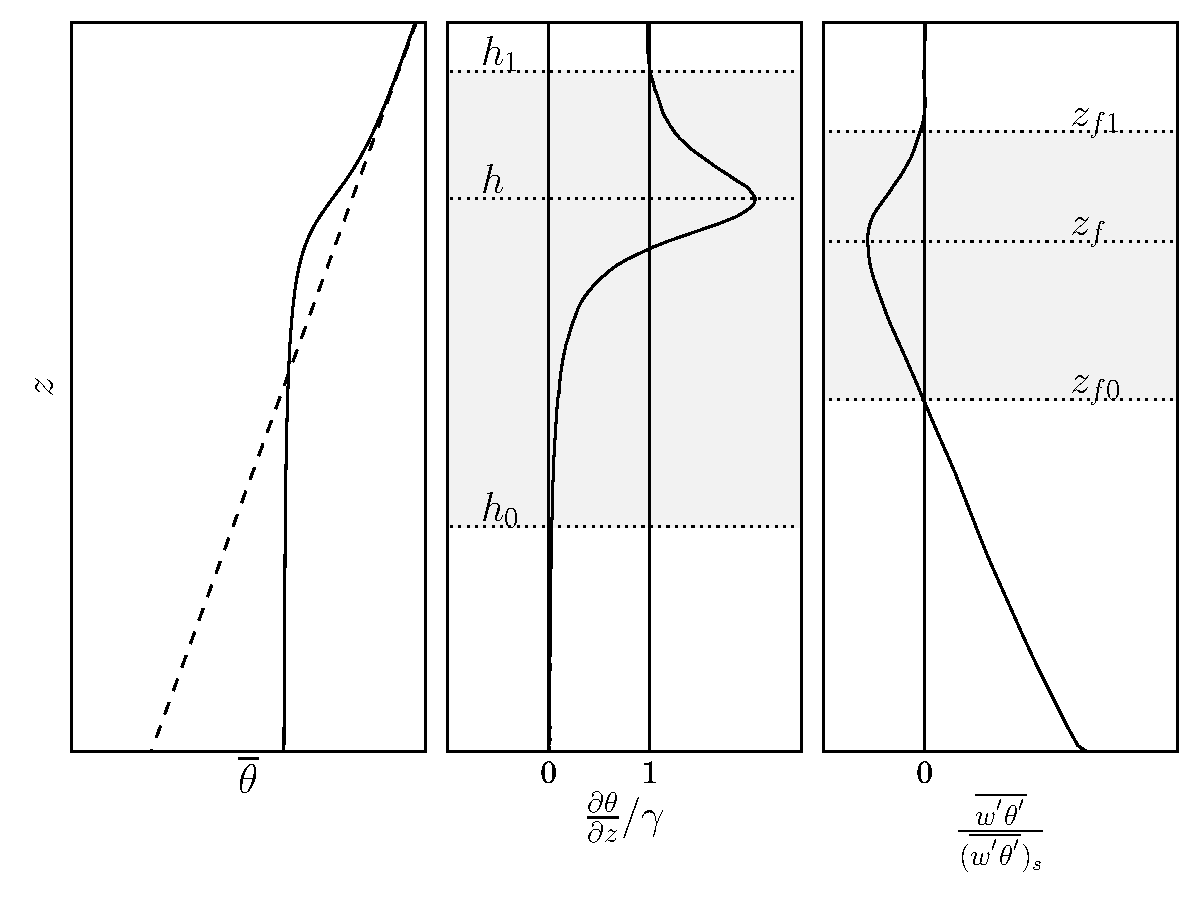
\includegraphics[scale=.5]{figures/height_defs.pdf}
    \caption[label a, b c Height Definitions]{Height definitions based on idealized scaled, averaged vertical profiles. a) dashed line: the initial potential temperature profile $\theta_0$,e solid: $\overline{\theta}$ at a later time. b)  $z_{f0}$, $z_{f}$ and $z_{f1}$ are the points at which the scaled vertical heat flux profile first crosses zero, is minimum and resumes zero. 
c)  $h$ is the location of the maximum scaled average potential temperature gradient, $h_{0}$ is the point at which $(\theta/dz)/\gamma$ increases significantly from zero and $h_{1}$ is where it returns to 1. The EZ is shaded.}
    \label{fig:hdefs} 
\end{figure}


\remarkpha{Add summary of: } \citet{Brooks12}, \citet{FedConzMir04}


\section{Scaling}

%pha --  change to flux since GM don't use gradient measure?

We follow \citep{Garcia14} and denote the surface buoyancy flux as $B_0 = g \overline{w^{'}\theta^{'}}_0/\overline{\theta}_0$ and the Brunt-Vaisala frequency as $N^2 = \gamma g/\theta_0$.
This energy and time scale yields a reference timescale of $N^{-1}$ and a length scale of $L_0=(B_0/N^3)^{1/2}$.  At high Reynolds numbers these two parameters determine the encroachement
depth as a function of time $t$ from an initial time $_0$:

\begin{equation}
  \label{eq:enc}
  z_{enc}(t) = \left [ \frac{2B_0}{N^2} (t - t_0) \right ]^{1/2}
\end{equation}

\cite{Garcia14} uses direct numerical simulation to show that, while the well knownn $z_{enc}$ is the effective scale for the middle of the entrainment zone ($h$ or $z_f$ in Figure~\ref{fig:hdefs}) there is a layer between $z_{enc}$ and the top of the entrainment zone with thickness that scales as:

\begin{equation}
  \label{eq:upper}
  \delta h \approx c_\delta (w_* / N )
\end{equation}
where $c_\delta \approx 0.55$.  This upper layer thickness $\delta h$ corresponds to  $z_{f1} - z_f$ or $h_1 - h$ in Figure~\ref{fig:hdefs}.
\remarkpha{show figure that demonstrates success of les in scaling this?}

The inversion strength $N$  enters the scaling for the upper region $\delta h$ because that thickness is governed by thermals impinging on the stable over-lying air.  
The lower layer the lower region, in which $z_f - z_{f0}$ scales with the CBL depth $h$  is comprised of mostly turbulent air with pockets of stable warmer air that are quickly mixed. 
We will show below that the flux and gradient definitions for the thickness of the lower layer $(z_{f} - z_{f0})$ and $h - h_0$ scale differently witn $N$ and $L_0$.
%remarkpha{mention this below}

Below we use large eddy simulation output to measure local and ensemble-averaged changes in the total EZ thickness $\Delta h$ and mixed layer depth $h$ as functions of surface heat flux and layer stability $\gamma$.  The convective Richardson number is a simplified, bulk approximation to the flux Richardson number \citep{Stull-BLMetIntro}.  The natural choice of length and velocity and temperature difference scales are $h$, $w_{*}$ and the jump across the -EZ, $\Delta \theta$:

\begin{equation}
Ri = \frac{\frac{g}{\overline{\theta}} \Delta \theta h}{w^{*2}}.
\end{equation}
whereas \cite{Sorbjan1} showed that with proximity to the CBL top the effects of FA stability $\gamma$ become more important.  An upper-level potential temperature scale for the EZ, $\delta h \gamma$, is demonstrated in Fig. \ref{fig:deltahgamma}. This is the difference in the initial or background potential temperature ($\overline{\theta}_{0}$) across the upper part of the EZ, i.e. between $h$ and $h_{1}$.\\      

A similar scale to $\delta h \gamma$ was introduced by \cite{Garcia14} to further their line of reasoning that the buoyancy in the upper EZ is determined by $\gamma$. A broad qualitative explanation is as follows: at $h$ much of the air is at the background (or initial) potential temperature $\overline{\theta}_{0}(h)$.  Some air at potential temperature $\theta = \overline{\theta}_{0}(h_{1})$ is brought down from the upper EZ limit ($h_{1}$) resulting in positive potential temperature fluctuations ($\theta^{'+}$) at $h$.\\

%plot_defs.py produces this on branch: deltah_gamma
\begin{figure}[htbp]
    \centering
    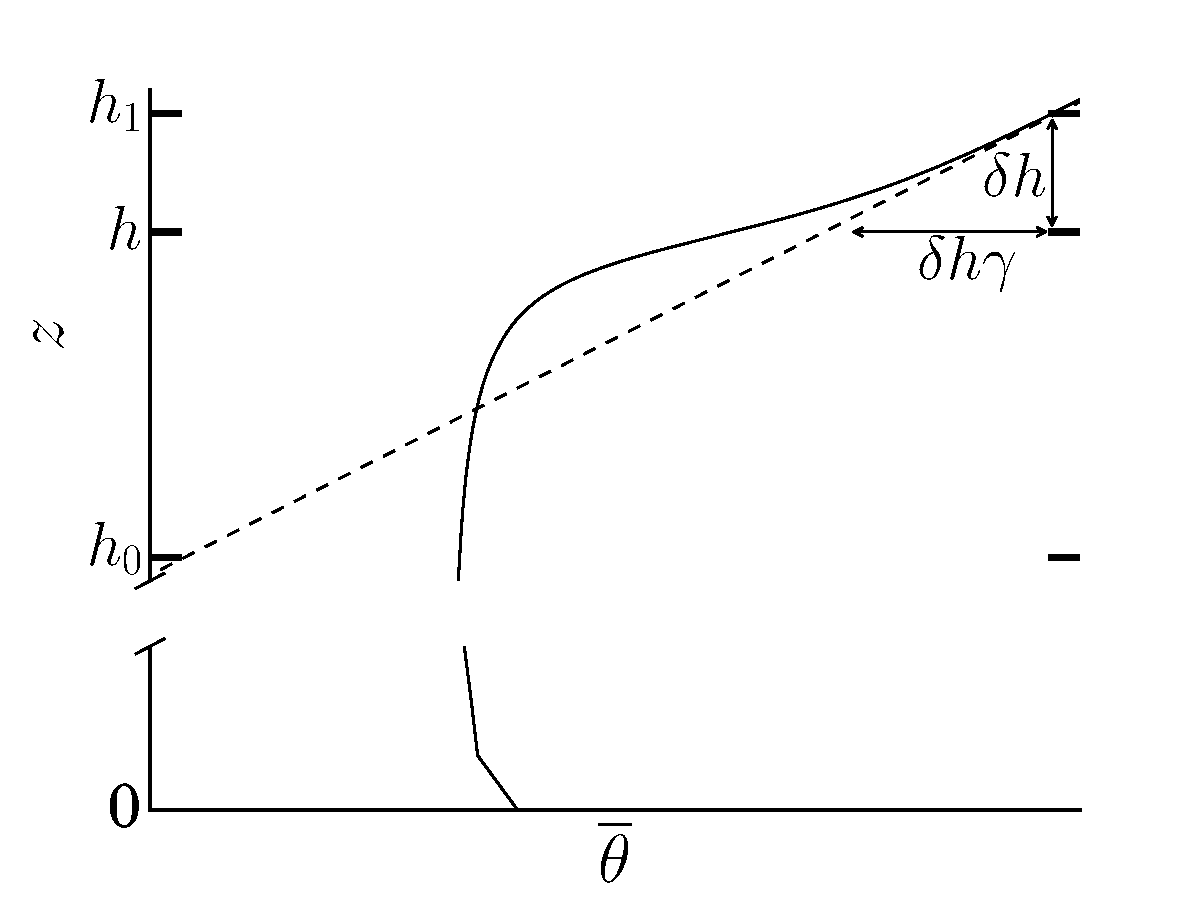
\includegraphics[scale=.32]{figures/deltah_gamma.pdf}
    \caption[Alternative Potential Temperature Scale for the EZ]{Representation of the difference in $\overline{\theta}_{0}$ across the upper part of the EZ, $\delta h \gamma$ where $\delta h = h_{1} - h$. This serves as an alternative to the convective potential temperature scale $\theta_{*}$.  The solid line is the average potential temperature profile and the dashed line is the initial or background potential temperature profile.}
    \label{fig:deltahgamma}   % label should change
\end{figure}

\subsubsection{Convective Richardson number ($Ri$)}
\label{subsubsec:}


$\Delta \theta$ can be replaced by the first order temperature jump, $\delta \theta$ as in \cite{FedConzMir04} and \cite{Garcia14}. 

\subsubsection{Relationship of entrainment zone depth to $Ri$}

A relationship of the scaled entrainment zone EZ depth to $Ri$

\begin{equation}\label{eq:dhvsri}
\frac{\Delta h}{h} \propto Ri ^{b}
\end{equation}

where $b=1$ is arrived at by considering the deceleration of a thermal
as it overshoots its neutral buoyancy level \cite{StullNelEl}.  Alternatively, \cite{Boers89} integrated the internal, potential and kinetic energy over a hydrostatic atmosphere to obtain a value of $b=\frac{1}{2}$.

\subsubsection{Relationship of entrainment rate to $Ri$}
\label{subsec:erri}
The relationship between scaled entrainment rate and the buoyancy Richardson number ($Ri$)

\begin{equation}\label{eq:ervsri}
\frac{w_{e}}{w_{*}} \propto Ri^{a}
\end{equation}
can be derived by integration of the conservation of enthalpy or turbulent kinetic energy equations over the growing CBL \citep{Tennekes73, Deardorff79, FedConzMir04}. It has been verified in numerous laboratory and numerical studies \citep{DearWill80, Sullivan98, FedConzMir04, Brooks12}, but there is still some unresolved discussion as the the exact value of a.  Simulations and observations give  values of the scaling exponent $a$ between $-\frac{3}{2}$ and $-1$ \citep{Traum11}.  \cite{Turner86} suggested that the former occurs at high stability when buoyant recoil of impinging thermals becomes more important than their convective overturning.  Adding further complexity to this discussion, \cite{FedConzMir04} arrived a similar power law relationship ($a = -1.7$) through defining the $\theta$ jump across the EZ ($\Delta \theta$) rather than at $h$ ($\delta \theta$).\\

Below we use a large eddy simulation to ...

\section{Tools and approach}

\subsection{LES set up}

The LES used in this study, System for Atmospheric Modeling (SAM)is an three-dimensional, anelastic model using dry static energy for its thermodynamic variable.  A Smagorinsky sub-grid scale closure was used for all simulations \citep{KhairRand}.

\subsubsection{Domain and grid sizes}
The dry shear free CBL and EZ was modeled using SAM.  An ensemble of 10 cases was run to obtain true ensemble averages and turbulent potential temperature fluctuations ($\theta^{'}$). Each case had a domain of area 3.2 x 4.8 km$^{2}$.  Grid numbers $n_{x}$, $n_{y}$ were chosen based on the optimal distribution across processor nodes. The vertical grid ($n_{z}=312$) was of higher resolution around the entrainment zone ($\Delta z = 5$m), lower below ($\Delta z = 25$m) and stretched above it ($\Delta z = 10 \ to \ 100 $m). This was guided by \cite{SullPat}'s LES resolution study of the CBL that showed how grid size effects the average profiles, as well as the extent of the inertial turbulence scale sub-range.\\

\subsubsection{Initial conditions}

The runs were initialized with a constant $(\overline{w^{'}\theta^{'}})_{s}$ acting against a uniform $\gamma$.  Thus, the  $\theta$ jump arose from the overshoot of the thermals, rather than being initially imposed as in \cite{Sullivan98} and \cite{Brooks12}.  The 7 runs differ from each other based on surface heat flux ( $(\overline{w^{'}\theta^{'}})_{s}$ ) and initial potential temperature lapse rate ($\gamma$) and are summarized accordingly in Table \ref{fig:tableofruns}.

\begin{table}[!ht]
\caption{Run parameters $\overline{w^{'} \theta^{'}_{s}}$, initial Lapse Rate $\gamma$ and Ozmidov depth $L_0$ (meters, in parenthesis).  This mapping between initial conditions and  plot symbols will be used in subsequent plots.}
    \begin{center}
    \begin{tabular}{ | l | l | l | l |}
    \hline
    $\overline{w^{'}\theta^{'}_{s}}$ / $\gamma$ & 10 (Kkm$^{-1}$) & 5 (Kkm$^{-1}$) & 2.5 (Kkm$^{-1}$) \\ \hline
     150 (Wm$^{-2}$)& \hspace{2mm} {\color{red} \ding{116}} 150/10 (29) &\hspace{3   mm}{\color{red} \ding{108}} 150/5 (48) \footnotemark &  \\ \hline
     100 (Wm$^{-2}$)& \hspace{2mm} {\color{black} \ding{116}} 100/10 (23) & \hspace{2mm} {\color{black} \ding{108}} 100/5 (39) & \\ \hline
     60 (Wm$^{-2}$) & \hspace{2mm} {\color{offyellow} \ding{116}} 60/10 (18) & \hspace{2mm} {\color{offyellow} \ding{108}} 60/5 (31) & \hspace{2mm} {\color{offyellow} \ding{72}} 60/2.5 \\
\hline
\end{tabular}
\label{fig:tableofruns}   
\end{center}    
\end{table}

\footnotetext{Incomplete run: EZ exceeded high resolution vertical grid after 7 hours}

\subsection{Comparison of domain, grid size and initial conditions}

\cite{SullPat} found that the shapes of the average potential temperature ($\overline{\theta}$) and heat flux ($\overline{w^{'}\theta^{'}}$) profiles, as well as the measured CBL height vary depending on grid size.  The resolution at which convergence began is listed in Table \ref{table:gridcomp}.  Lower resolution resulted in a higher CBL and relatively larger EZ based on the $\overline{\theta}$ and $\overline{w^{'}\theta^{'}}$ profiles.  Overall they concluded that vertical resolution was critical.  This compliments the conclusion \cite{Brooks12} reached when discussing their resolution test.  That is, to capture the steep vertical gradients in the EZ requires high vertical resolution. \\

Fast Fourier transform (FFT) energy spectra of the turbulent velocities at the top of the ML (not shown) show a substantial resolved inertial subrange giving confidence in the choice of horizontal grid size used. In the EZ where turbulence is intermittent, the dominant energy containing structures are smaller, and decay to the smallest resolved turbulent structures is steeper. Two dimensional horizontal slices of potential temperature and turbulent vertical velocity perturbations at $h_{0}$, $h$ and $h_{1}$ show several coherent impinging thermals at any given time after 2 hours, indicating that realistic turbulence was being simulated \ref{nchap14}.\\

\begin{table}[htbp]
\caption[Comparison of Grid-Sizes used in similar Studies]{Grid spacing around the EZ used in comparable LES studies. Those used for resolution tests are not listed here.  For \cite{SullPat}'s resolution study the grid sizes, at which profiles within the EZ and CBL height evolution began to converge, are listed.}

    \begin{tabular}{p{4cm} p{2cm} p{2cm}}
Publication & $\Delta x$, $\Delta y$, $\Delta z$ & Horizontal \\
 & in the EZ (m) & Domain (km$^{2}$) \\ \hline
      \cite{Sullivan98}& 33, 33, 10 & 5 x 5 \\ 
      \cite{FedConzMir04}& 100, 100, 20 & 5 x 5 \\ 
      \cite{Brooks12}& 50, 50, 12 & 5 x 5 \\
      \cite{SullPat} &  20, 20, 8 & 5 x 5\\
      This study & 25, 25, 5 &  3.4 x 4.8\\ \hline       
    \end{tabular}
%}
\label{table:gridcomp}   
%\end{center}    
\end{table}

Move?

The principal parameter describing the balance of forces in dry, idealized CBL entrainment is the Richardson number ($Ri$) and its magnitude depends on the way in which the $\theta$ jump is defined.  Varying the $\theta$ jump definition causes identical conditions to be described by different $Ri$ values.  In this study the dependence of $Ri$ on variation in $\gamma$ was evident.  \cite{Brooks12} and \cite{Sullivan98} imposed a $\theta$ jump of varying strength topped by a constant $\gamma$.  Whereas \cite{FedConzMir04} initialized with a layer of uniform $\theta$.  They varied $\gamma$ and kept $\overline{w^{'}\theta^{'}}_{s}$ constant for each run.  Their initial conditions, definitions of the $\theta$ jump and $Ri$ range are directly comparable to those of this study.  \cite{Brooks12} and \cite{Sullivan98} defined CBL height, the EZ and $\theta$ jump as averages of local values determined based on tracer profiles.  So the resulting $Ri$ values are quite different.    

\begin{table}[htbp]
\caption[Initial Conditions used in comparable LES Studies]{Initial Conditions used in comparable LES Studies}

  
    \begin{tabular}{ p{4cm} p{1.4cm} p{1.4cm} p{1.7cm} p{1.8cm}}
    
Publication & $\overline{w^{'}\theta^{'}}_{s}$& $\gamma$& Initial $\theta$ & $Ri$ \\ 
& $Wm^{-2}$ & $Kkm^{-1}$ & Jump K & range \\ \hline
      \citeauthor{Sullivan98} (\citeyear{Sullivan98}) & 20 - 450& 3  &.436 - 5.17 & 1 - 100\\
      \citeauthor{FedConzMir04} (\citeyear{FedConzMir04}) & 300 & 1 - 10 & NA & 10 - 40\\ 
      \citeauthor{Brooks12} (\citeyear{Brooks12}) &  10 -100 &  3& 1 - 10 &10 - 100 \\
      This study & 60 - 150 & 2.5 - 10& NA & 10 - 30\\ \hline 
      
    \end{tabular}
%}
\label{table:initconditcomp}   

\end{table}

\subsection{Tri-linear fit for local CBL height}
\cite{Sullivan98} determined local CBL height, i.e. that at an individual horizontal point, by locating the point of maximum $\frac{\partial \theta}{\partial z}$.  Analysis of the resulting distributions showed dependence of standard deviation and skewness on $Ri$.  The normalized standard deviation decreased with increased $Ri$ whereas skewness was almost bimodal; being negative at high $Ri$ and positive and low $Ri$.  Initially in this study, a similar method was applied and local CBL height distributions with lower $Ri$ were found to have positive skew.  Upon exhaustive inspection of local vertical $\theta$  profiles such as those in Fig. \ref{fig:rssfitshigh}, it became evident that at certain horizontal points high gradients well into the free atmosphere exceeded those within the EZ.  Locating the local ML height ($h^{l}_{0}$) using a multi-linear regression method based on that of \citep{Vieth} and described in \cite{nchap14} proved more reliable than the gradient method discussed above.  As shown in Fig. \ref{fig:rssfitshigh} a straight line is fit to each of the ML, EZ an FA.\\
  
\begin{figure}[htbp]
\begin{minipage}[b]{0.5\linewidth}
        %Pcolor_Peaks.py on branch rss_fit, using IPython QtConsole 3.1.0 Python 2.7.9 |Anaconda 2.2.0 (64-bit)|
        \subfloat[]{\label{main:a}
                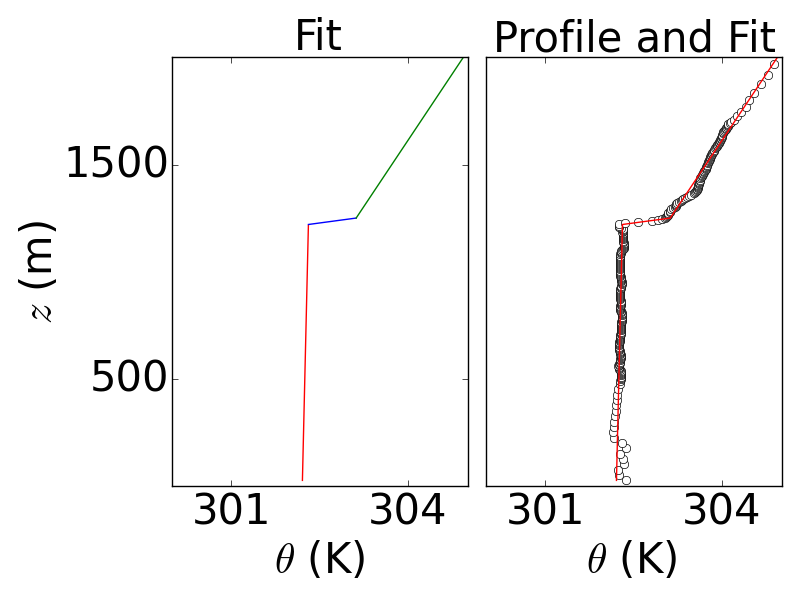
\includegraphics[scale=.31]{figures/rss_fit_high}}\\
        \end{minipage}             
\quad
\begin{minipage}[b]{0.5\linewidth}
        \subfloat[]{\label{main:b}          
                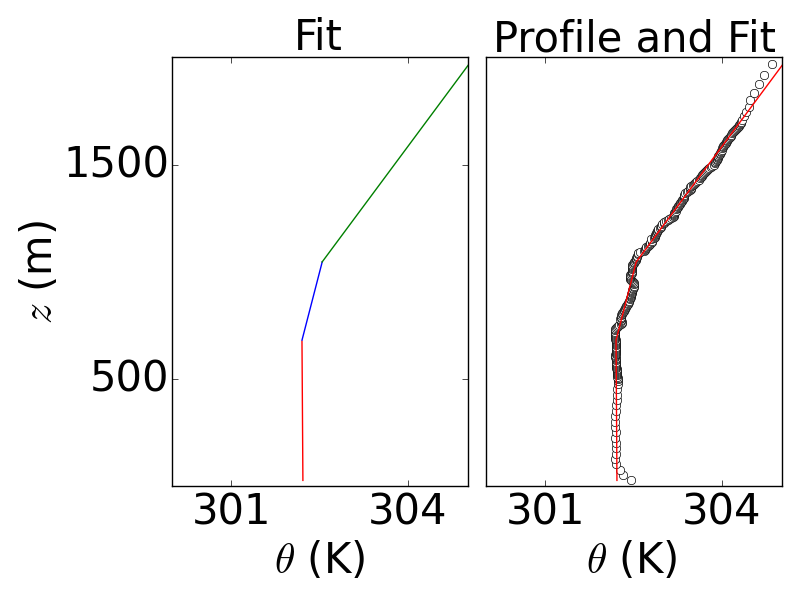
\includegraphics[scale=.31]{figures/rss_fit_low}}\\       
       \end{minipage}
\caption[High local ML ]{Local vertical $\theta$ profiles with tri-linear fit for the 60/2.5 run at a point where $h^{l}_{0}$ (a) is high and (b) low.}
\label{fig:rssfitshigh}
\end{figure}

\subsection{Definitions based on scaled ensemble and horizontally averaged profiles}

Here the CBL height ($h$) is defined as the location of maximum scaled vertical $\overline{\theta}$ gradient as in Figure \ref{fig:hdefs}.  The lower and upper EZ boundaries ($h_{0}$ and $h_{1}$) are then the points at which $\frac{\frac{\partial \overline{\theta}}{\partial z}}{\gamma}$ significantly exceeds zero and where it resumes $1$.  The lower boundary requires a choice of a threshold value which should be small, positive and less than $1$. \cite{FedConzMir04} and \cite{Brooks12} defined the EZ in terms of the vertical $\overline{w^{'}\theta^{'}}$ profiles as in Figure \ref{fig:hdefs} but disagreed on the shape of the relationship of scaled EZ depth to $Ri$ (equation 2.1).  As well as observing this relationship using the height definitions based on the $\frac{\frac{\partial \overline{\theta}}{\partial z}}{\gamma}$ profile, definitions based on the $\frac{\overline{w^{'}\theta^{'}}}{(\overline{w^{'}\theta^{'}})_{s}}$ profile are applied to enable comparison with \cite{Brooks12}, \cite{FedConzMir04} and \cite{Garcia14}.\\  

\begin{table}[htbp]
\caption[Height definitions]{Definitions based on the vertical $\overline{\theta}$ profile in Figure \ref{fig:hdefs}. $\delta \theta$ and $\Delta \theta$ are the temperature jumps corresponding to the zero and first order models respectively. To obtain those based on the $\overline{w^{'}\theta^{'}}$ profile, replace $h_{0}$, $h$ and $h_{0}$ with $z_{f0}$, $z_{f}$ and $z_{f1}$}


    \begin{tabular}{p{1.cm} p{3.cm} p{3cm} p{2.5cm}}
    
      CBL Height & ML $\overline{\theta}$ & $\theta$ Jump &$     Ri $\\ \hline 
       $h$ & $\overline{\theta}_{ML} = \frac{1}{h}\int^{h}_{0}\overline{\theta}(z)dz$ & $\Delta \theta=\overline{\theta}(h_{1})-\overline{\theta}(h_{0})$ &      Ri $_{\Delta}=\frac{\frac{g}{\overline{\theta}_{ML}}\Delta \theta h}{w^{*2}}$  \\ [.3cm] 
        
       & &$\delta \theta = \overline{\theta}_{0}(h)- \overline{\theta}_{ML}$ & \    Ri $_{\delta}=\frac{\frac{g}{\overline{\theta}_{ML}} \delta \theta h}{w^{*2}}$ \\ \hline
      \end{tabular}

\label{tab:reldefs}   
    
\end{table}

\section{Results}
\subsection{Entrainment zone structure}

\subsubsection{Variation of local convective boundary layer height ($h_{0}^{l}$)}
\label{subsubsec:loccblh}


The distribution of $h_{0}^{l}$ represents the range over which CBL height varies in space so relates to the depth of the entrainment zone (EZ).  It widens with increasing $(\overline{w^{'}\theta^{'}})_{s}$ and narrows with increasing $\gamma$ \citep{nchap14}.  When scaled by $h$ in Fig. \ref{fig:localhdist}, the local ML height distribution narrows with increased $\gamma$.  The upper boundary seems to be constant at about 1.1($\times h$) , whereas the lower boundary increases.  When $h_{0}^{l}$s are lower and their distribution is narrower, the scaled versions have relatively larger spacing between bins and so higher numbers in each bin. At higher $(\overline{w^{'}\theta^{'}})_{s}$ there are fewer $\frac{h_{0}^{l}}{h}$ values with higher probabilities, but the width of the distributions seems more or less constant regardless of $(w^{'}\theta^{'})_{s}$.\\


\begin{figure}[htbp]
%ML_Height_Hist.py on branch: ML_Height_hist_5
        \begin{center}
        \subfloat[]{\label{main:}
                %45e344 (commit)
                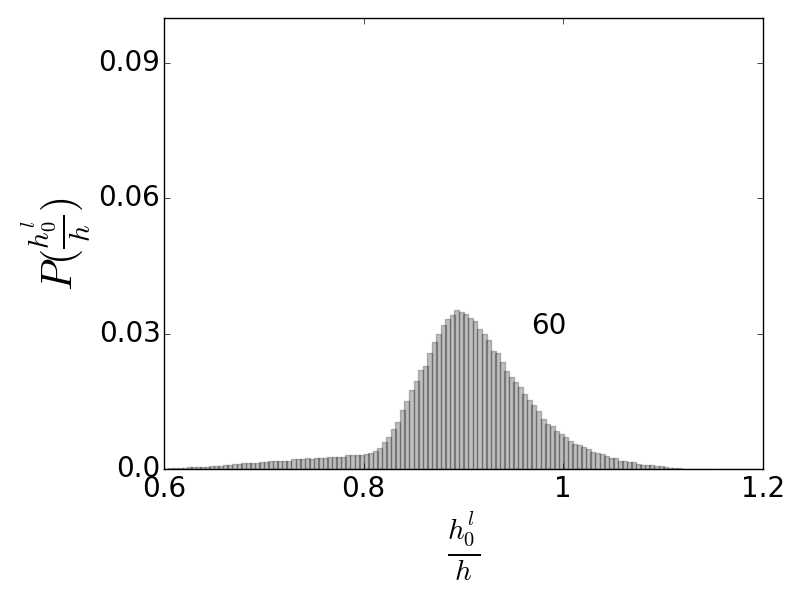
\includegraphics[scale=.3]{figures/Scaled_ML_Height_hist_2point5}}\\
\end{center}
\quad
\begin{center}
        \subfloat[]{\label{main:}        
                %02c9b5 (commit)
                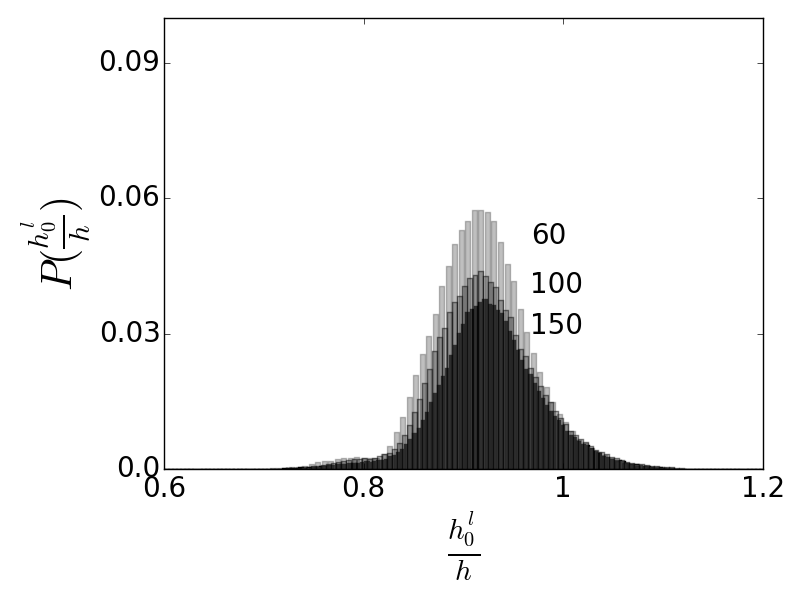
\includegraphics[scale=.3]{figures/Scaled_ML_Height_hist_5}}\\      
\end{center}         
\quad
\begin{center}
        \subfloat[]{\label{main:}          
               %4a72ab (commit)
                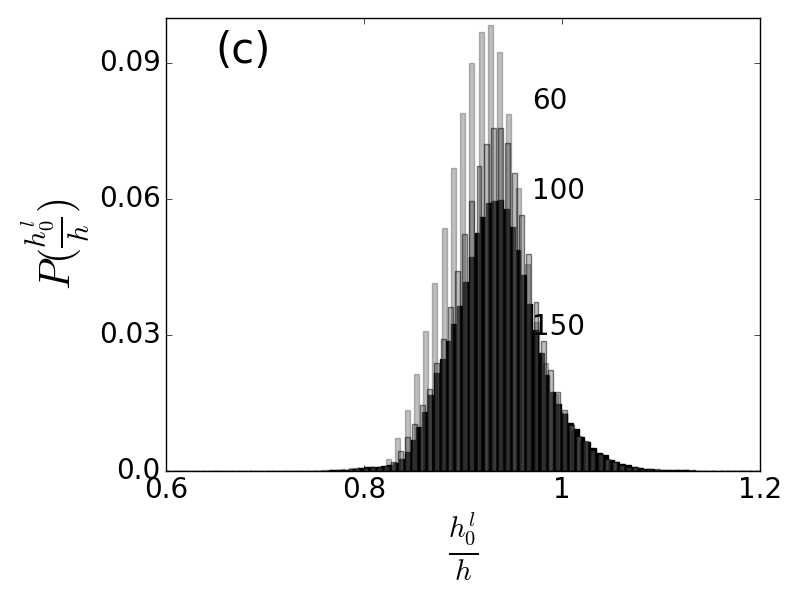
\includegraphics[scale=.3]{figures/Scaled_ML_Height_hist_10}}\\      
\end{center}       

        \caption[Local Scaled ML Height Distributions]{Probability distributions of scaled local ML heights ($\frac{h^{l}_{0}}{h}$) for $\gamma = 2.5$ Kkm$^{-1}$ (a), $\gamma = 5$ Kkm$^{-1}$ (b) and $\gamma = 10$ Kkm$^{-1}$ (c). Darker shading corresponds to higher $(\overline{w^{'}\theta^{'}})_{s}$, i.e. $60 - 150$ Wm$^{-1}$ per plot annotation.  The probabilities are the proportions in each scaled height bin. All plots are of output at 5 simulated hours.}
    
        \label{fig:localhdist}
\end{figure}

The lowest $\frac{h^{l}_{0}}{h}$ decrease with decreased stability ($Ri$) causing increased negative skew. This, combined with a widening of the distribution agrees, with the findings of \cite{Sullivan98} and supports the results based on the average profiles to be discussed later. \\  

\subsubsection{Downward moving warm air at $h$}
\label{subsubsec:downwarm}

\cite{Sullivan98} separated the vertical heat flux in the EZ into four quadrants: upward moving warm, downward moving warm, upward moving cool and downward moving cool. They concluded that the net transport in the EZ was determined by downward moving warm air. The LES simulations show that the average downward moving warm quadrant ($\overline{w^{'-}\theta^{'+}}$) at $h$ represents the pockets of trapped or engulfed warm air that become mixed into the growing CBL.  So its magnitude can be taken as a measure of entrainment.  This increases in magnitude, with time as well as with increasing $(\overline{w^{'}\theta^{'}})_{s}$ \citep{nchap14}.  Partitioning $(\overline{w^{'-}\theta^{'+}})_{h}$ into its velocity and temperature components reveals complexity.  The velocity component, $\overline{w^{'-}}_{h}$  where $ \overline{\theta^{'}}_{h}>0$, is effectively scaled by $w_{*}$.  The curves representing the temperature component, $\overline{\theta^{'+}}_{h}$ where $\overline{w^{'}}_{h}<0$, vs time do not seem to collapse when scaled by $\theta_{*}$ \citep{NChap14}.  Fig. \ref{fig:downwarm_theta} (a) shows this component is scaled more effectively by the potential temperature scale introduced in Section \ref{subsubsec:tempscales}, $\delta h \gamma$.  Thus, $\gamma$ influences entrained warm air at $h$ more significantly than $(\overline{w^{'}\theta^{'}})_{s}$.\\ 
\\   
%plot_downwarm_h.py on branch downwarm
\begin{figure}[htbp]
%b5557c9 (commit)
\begin{minipage}[b]{0.5\linewidth}
         \subfloat[]{\label{main:a}
                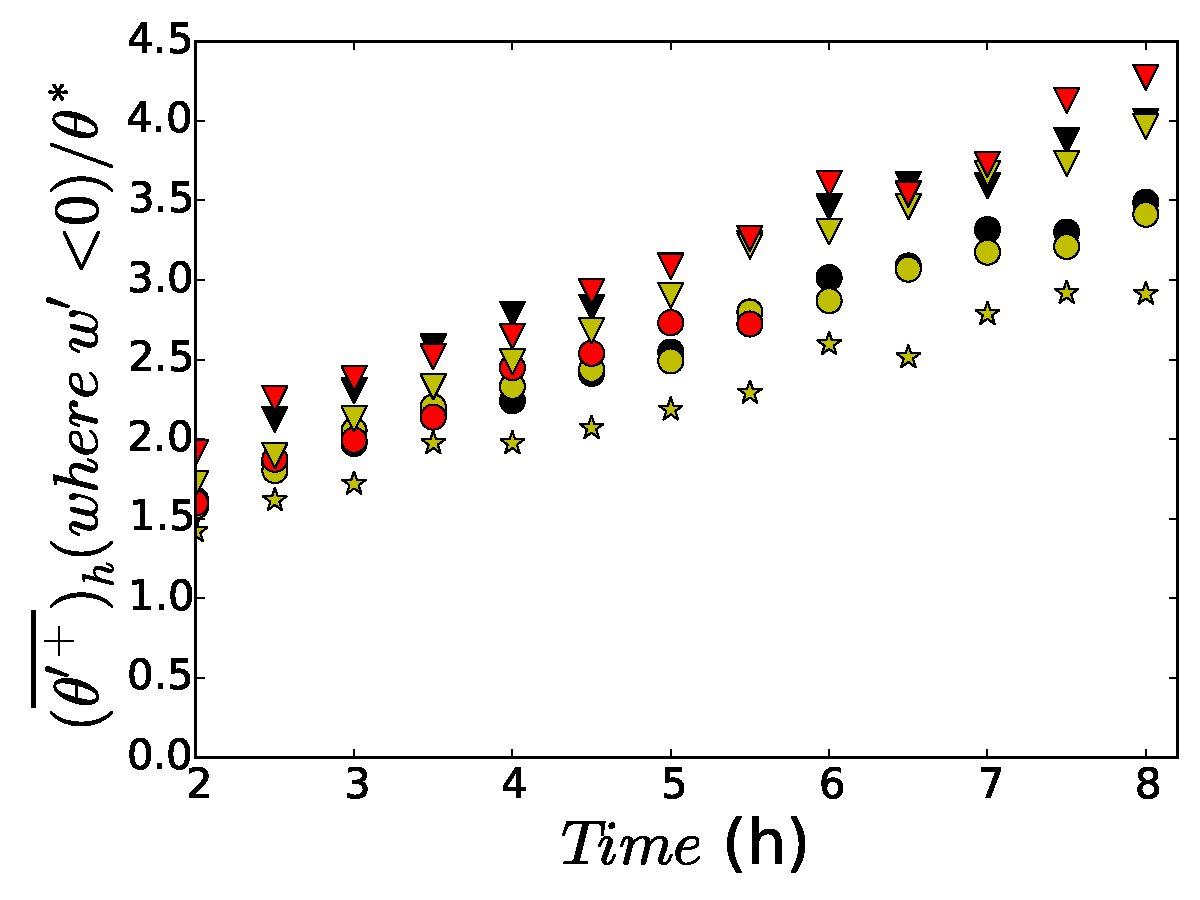
\includegraphics[scale=.3]{figures/scaled_downwarm_theta.pdf}}\\
                     
\end{minipage}             
\quad
%772a9 (commit)
\begin{minipage}[b]{0.5\linewidth}
         \subfloat[]{\label{main:b}          
               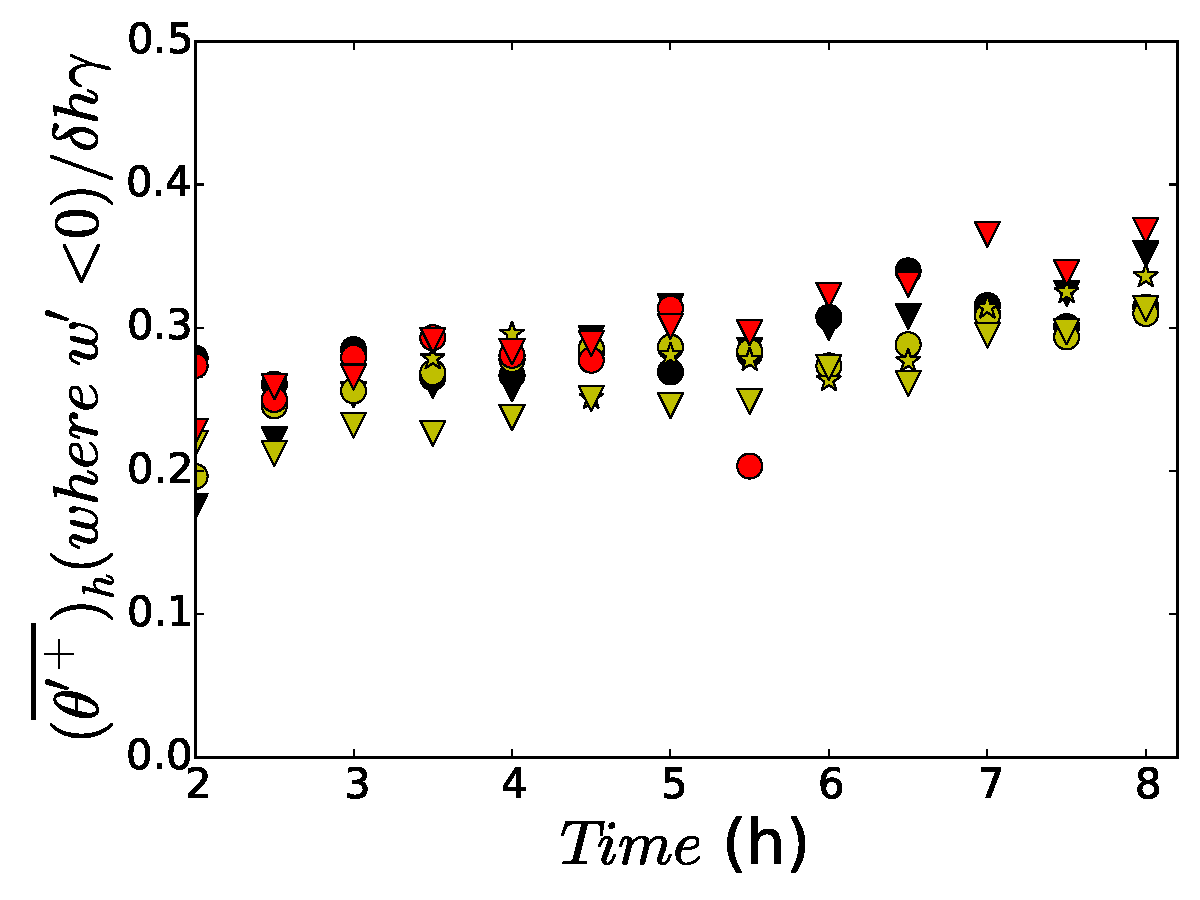
\includegraphics[scale=.3]{figures/scaled_downwarm_theta1.pdf}}\\      
       
        \end{minipage}
        \caption[Downward moving positive potential temperature fluctuations at $h$]{(a) shows $\overline{\theta^{\prime+}}_{h}$ at points where $w^{\prime}<0$ and (b) $\overline{\theta^{\prime+}}_{h}$ where $w^{\prime}<0$ scaled by $\delta h \gamma$.  Legend key:{\color{red} \ding{116}} 150/10 \hspace{3mm}{\color{red} \ding{108}} 150/5 \hspace{2mm} {\color{black} \ding{116}} 100/10 \hspace{2mm} {\color{black} \ding{108}} 100/5 \hspace{2mm} {\color{offyellow} \ding{116}} 60/10 \hspace{2mm} {\color{offyellow} \ding{108}} 60/5 \hspace{2mm} {\color{offyellow} \ding{72}} 60/2.5}
        \label{fig:downwarm_theta}
\end{figure}
\clearpage

\subsection{EZ boundaries}

%\subsubsection{Height definitions based on scaled $\overline{w^{'}\theta^{'}}$}

\subsubsection{Heights based on scaled $\overline{\theta}$ gradient profile}

Figure 6 shows ...

Initially, CBL height and EZ boundaries are defined based on the (unscaled) $\frac{\partial \overline{\theta}}{\partial z}$ profile. A threshold value for the lower EZ boundary ($h_{0}$) was chosen here, such that it was positive, small (i.e. an order of magnitude less than $\gamma$) and the same for all runs.  For the sake of rigor, plots of Eq. \ref{eq:dhvsri} are produced based on two additional threshold values yielding analogous results \citep{NChap14}.  In all three cases curves group according to $\gamma$ as shown in Fig. \ref{fig:scaleddeltahinvri} (c).\\

The importance of $\gamma$ is revealed again as the curves representing Equation \ref{eq:dhvsri} in Fig. \ref{fig:scaleddeltahinvri} (d) become similar when heights are based on the scaled profile, $\frac{\frac{\partial \overline{\theta}}{\partial z}}{\gamma}$ shown in Fig. \ref{fig:scaleddeltahinvri}. Closer inspection shows that this change primarily occurs at the lower EZ boundary ($h_{0}$) when $\frac{\partial \overline{\theta}}{\partial z}$ is scaled by $\gamma$. So the upper, or initial, lapse rate influences both the vertical temperature gradient at the lower EZ boundary and the downward moving warm air at the CBL top.\\

\begin{figure}[htbp]
\begin{minipage}[b]{0.5\linewidth}
        %branch: master, plot_theta_profs.py, 04cb3b  
        \subfloat[]{\label{main:}
                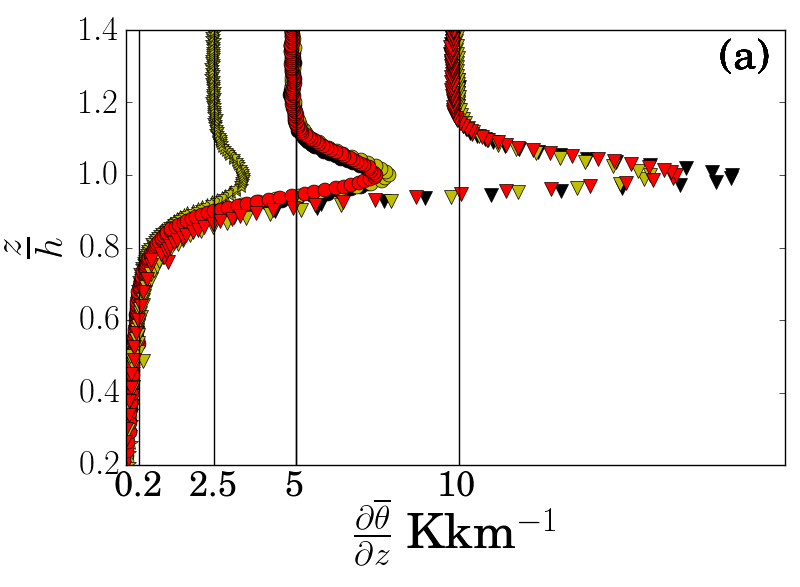
\includegraphics[scale=.3]{figures/theta_grad_profs}}\\
%        \subfloat[]{\label{main:}
%                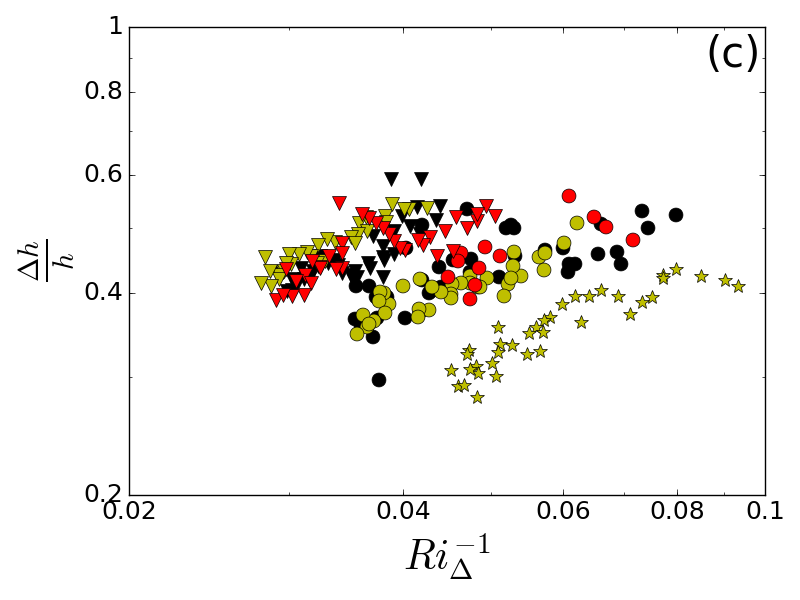
\includegraphics[scale=.3]{figures/scaleddeltahinvri}}\\
                     
\end{minipage}             
\quad
\begin{minipage}[b]{0.5\linewidth}
        \subfloat[]{\label{main:}        
         %branch: master, plot_theta_profs.py, 96c220
                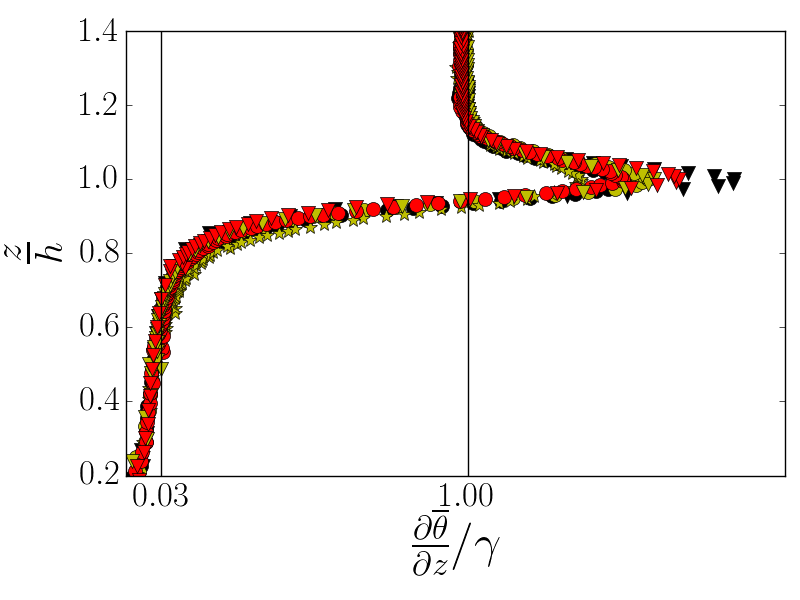
\includegraphics[scale=.3]{figures/scaled_theta_grad_profs}}\\      
%        \subfloat[]{\label{main:}          
          
%                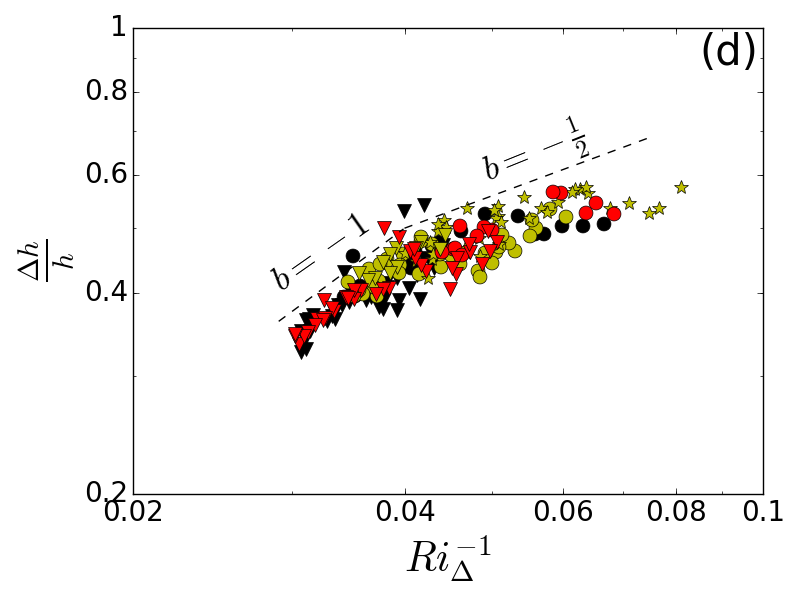
\includegraphics[scale=.3]{figures/loglog_scaleddeltahinvri_4}}\\      
       
\end{minipage}
\begin{minipage}[b]{0.5\linewidth}
%run get_limits.py then plot_height.py on branch scaleddeltahinvri         
%        %branch: scaleddeltahinvri_for_old_els, get_limits.py and plot_height.py
%                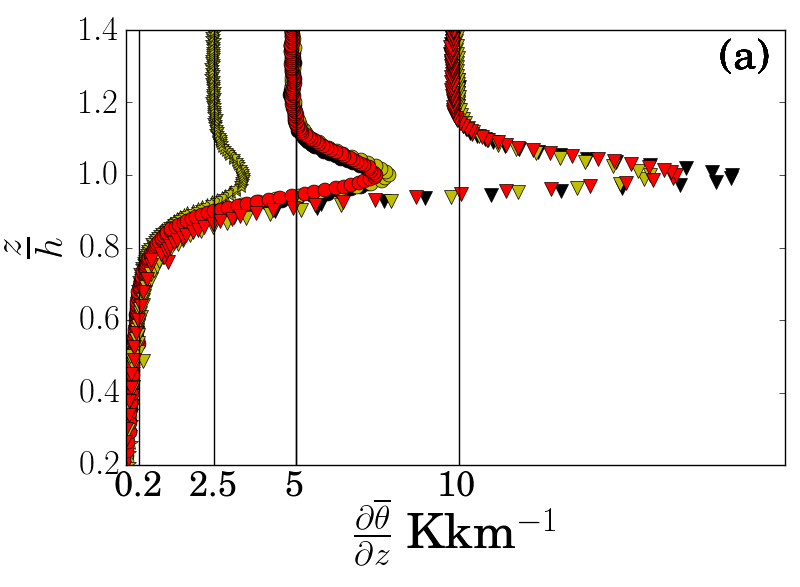
\includegraphics[scale=.3]{figures/theta_grad_profs}}\\
        \subfloat[]{\label{main:}
                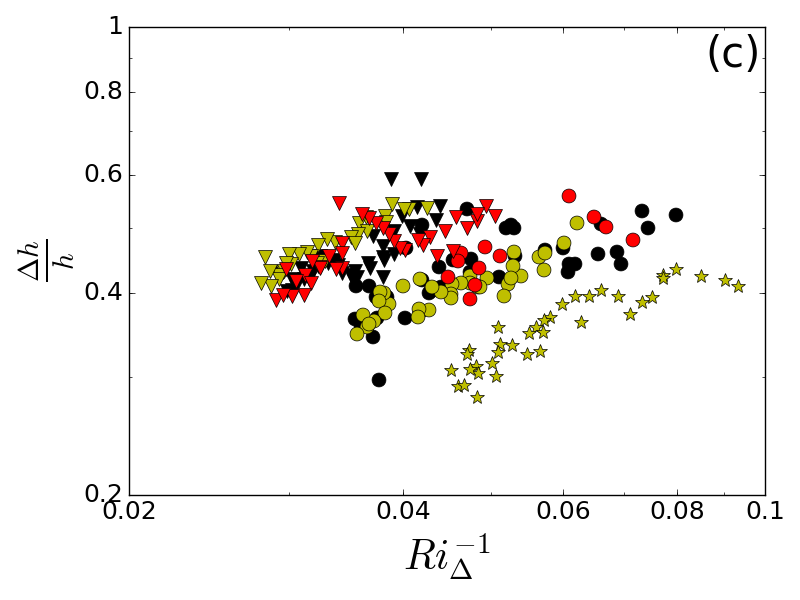
\includegraphics[scale=.3]{figures/scaleddeltahinvri}}\\
                     
\end{minipage}             
\quad
\begin{minipage}[b]{0.5\linewidth}
%        \subfloat[]{\label{main:}        
%run get_limits.py on branch: plot_defs, 8d1fab (commit), then plot_height.py on branch: loglogscaleddektahinvri         
%                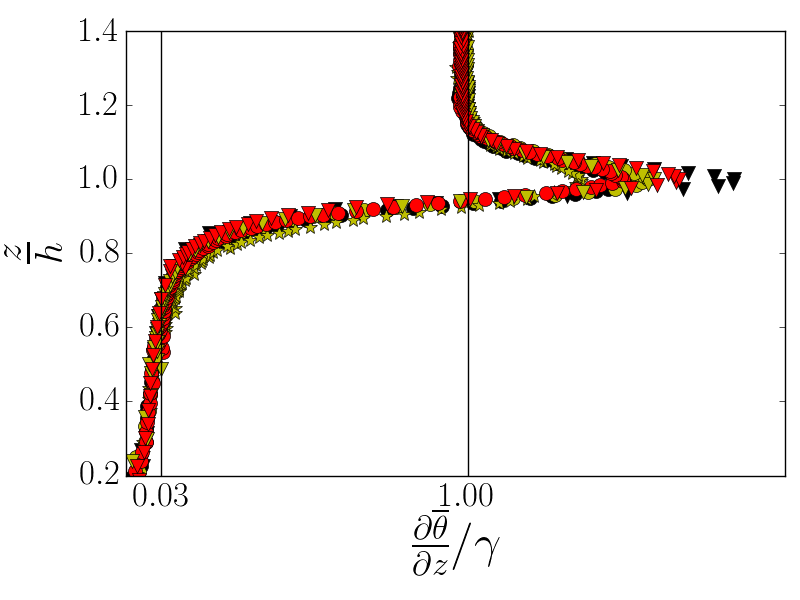
\includegraphics[scale=.3]{figures/scaled_theta_grad_profs}}\\      
        \subfloat[]{\label{main:}          
          
                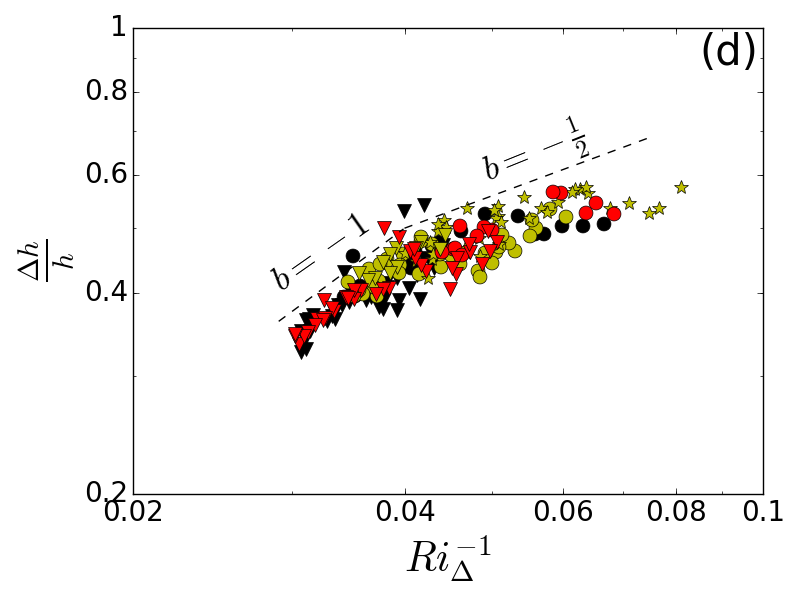
\includegraphics[scale=.3]{figures/loglog_scaleddeltahinvri_4}}\\      
       
        \end{minipage}

        \caption{The average (unscaled) vertical potential temperature gradient profiles for each run are plotted in (a) for comparison with the scaled versions ($\frac{\partial \overline{\theta}}{\partial z}/\gamma$) in (b). Solid lines show the thresholds, $\frac{\partial \overline{\theta}}{\partial z}=2$Kkm$^{-1}$ and $\frac{\partial \overline{\theta}}{\partial z}/\gamma=0.03$ respectively, used for determining the lower EZ boundary.  The corresponding plots of $\frac{\Delta h}{h} \propto Ri_{\Delta} ^{b}$ are plotted in log-log coordinates in (c) and (d) to show how curves separate according to $\gamma$ when heights are based on the unscaled profile, and collapse when based on the scaled version.  Legend key:{\color{red} \ding{116}} 150/10 \hspace{3mm}{\color{red} \ding{108}} 150/5 \hspace{2mm} {\color{black} \ding{116}} 100/10 \hspace{2mm} {\color{black} \ding{108}} 100/5 \hspace{2mm} {\color{offyellow} \ding{116}} 60/10 \hspace{2mm} {\color{offyellow} \ding{108}} 60/5 \hspace{2mm} {\color{offyellow} \ding{72}} 60/2.5.}
        \label{fig:scaleddeltahinvri}
\end{figure}


These results support a varying exponent $b$ in Equation \ref{eq:dhvsri} which is lower in magnitude ($-\frac{1}{2}$) at lower $Ri$ and approaches $-1$ at higher $Ri$.  This is in line with theory and the results of comparable studies so the EZ boundary definitions based on the $\frac{\frac{\partial \overline{\theta}}{\partial z}}{\gamma}$ profile are valid.  Overall there is a clear narrowing of the scaled EZ depth with increasing $Ri$ (decreasing $Ri^{-1}$) as supported by the local height distributions in Section \ref{subsubsec:loccblh}.  Although based on different height definitions, \cite{FedConzMir04} concluded an exponent $b = -\frac{1}{2}$ and \cite{Brooks12}'s plots show curves with an apparent exponent less in magnitude than $-1$.  Their curves representing each run fanned out.  Here, before scaling by $\gamma$, the curves representing Eq. \ref{eq:dhvsri} using height definitions based on $\frac{\partial \overline{\theta}}{\partial z}$ separate out, but in the reverse order.  Increased stability, ie higher $Ri$, causes larger scaled EZ depths.  Whereas \cite{Brooks12}'s runs with initially lower $Ri$ had larger scaled EZ depths than those with higher, even where $Ri$ values overlap. Nonetheless, that there appears a family of separate but similar curves rather than a single curve hints at an aditional underlying scaling parameter.\\     

\cite{Garcia14} suggested that the buoyancy in the lower portion of the EZ, i.e. from a point just below $h$ down, is more strongly influenced by the vigorous turbulence of the ML than by $\gamma$.  So mixing reduces the difference between, the potential temperature at the top of the ML, and that at or just below $h$.  However, that the magnitude of the average vertical potential temperature gradient ($\frac{\partial \overline{\theta}}{\partial z}$) in the upper ML increases with increasing $\gamma$, indicates that the influence of this parameter extends further down.\\

It is possible that the change in exponent with increased $Ri$ observed in Fig. \ref{fig:scaleddeltahinvri} (d) represents a change in entrainment mechanism. \cite{Sullivan98} observed enfolding and engulfment at lower $Ri$.  Whereas at higher $Ri$ when motion is more restricted, entrainment seemed to occur via trapping of thinner wisps at the edge of an upward moving thermal.  \cite{Turner86} also distinguishes between entrainment by convective overturning and recoil. \cite{Garcia14} refer to a change in entrainment rate due to the effects of increased stability on the upper EZ sub-layer.  In this study, the narrowing of the EZ depends predominantly on the magnitude of the average vertical potential temperature gradient $\frac{\partial \overline{\theta}}{\partial z}$ in the lower EZ and upper ML.  However, the scaled magnitude of upper limit does appear to decrease slightly in time.  This could correspond to the slowly decreasing upper sub layer of the EZ mentioned in both \cite{Garcia14} and \cite{FedConzMir04}.\\

The scaled EZ depth defined based on the vertical heat flux profile ($\frac{z_{f0}-z_{f1}}{z_{f}}$), remains more less constant with respect to time and shows little or no $Ri$ dependence.  This is supported by the similarity in time and across runs of the vertical heat flux profiles when scaled by $(\overline{w^{'}\theta^{'}})_{s}$ \citep{NChap14}.

\subsection{Entrainment rate}

$Ri$ magnitude determined in this and the comparable studies is primarily influenced by the magnitude of the $\theta$ jump.  Here it is defined in two ways, $Delta \theta$ and $\delta \theta$, as \cite{FedConzMir04} did.  The heights and $\theta$ jump are based on the scaled $\overline{w^{'}\theta^{'}}$ profile aswell as the scaled $\overline{\theta}$ gradient profile (Figure \ref{fig:hdefs} and Table \ref{tab:reldefs}).  This multitude of definitions enables comparison and observation of how the $\theta$ jump definition effects the exponent of Eq. \ref{eq:ervsri}.

\subsubsection{Height definitions based on scaled $\overline{w^{'}\theta^{'}}$}
In Fig. \ref{fig:weinvri} (a) and (b) the axes are in log-log coordinates and all heights are based on the scaled $\overline{w^{'}\theta^{'}}$ profile.  \cite{Garcia14} interpreted both curves as asymptotic to straight lines ($a=-1$) as the upper EZ sub-layer narrows.  These straight lines are plotted in Fig. \ref{fig:weinvri} (a) and (b) indicating that their DNS results have been reproduced here.   Plot (a) for $\delta \theta$ in Figure \ref{fig:weinvri} could also represent a curve with exponent less in magnitude than $-1$ initially.  Plot (b) for $\Delta \theta$ could represent a curve with increasing exponent exceeding magnitude $-1$ at higher $Ri$.\\

\begin{figure}[htbp]
\begin{minipage}[b]{0.5\linewidth}
        %98568f get_limits.py and plot_height.py
        \subfloat[]{\label{main:a}
                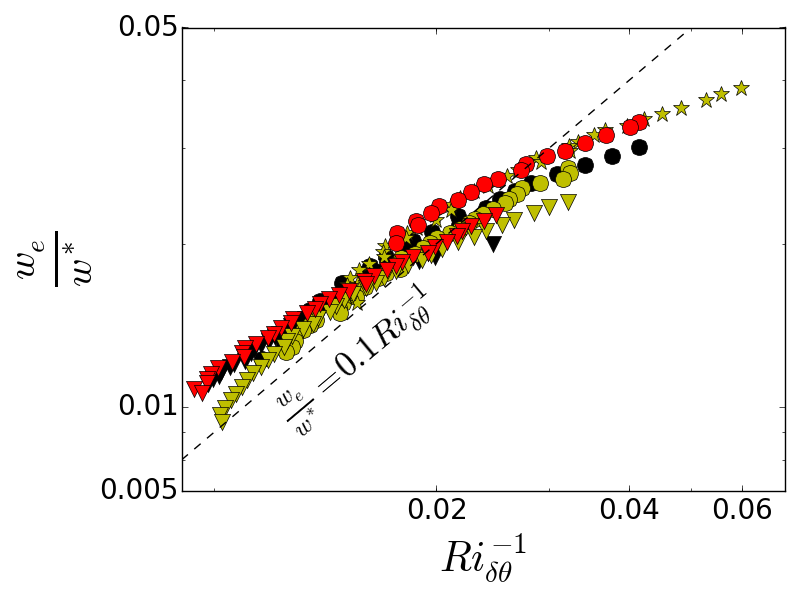
\includegraphics[scale=.3]{figures/scaledweinvri_delta_f_GM.png}}\\
%        \subfloat[]{\label{main:b}
 %               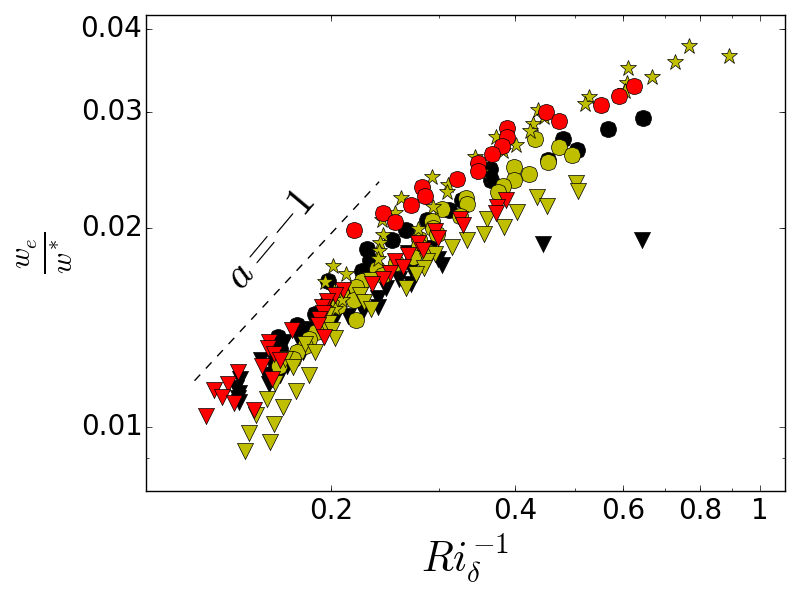
\includegraphics[scale=.3]{figures/scaledweinvri_delta.png}}\\
                     
\end{minipage}             
\quad
\begin{minipage}[b]{0.5\linewidth}
  %e4477b get_limits.py, ef6bfa plot_height.py      
  %      \subfloat[]{\label{main:a}
   %             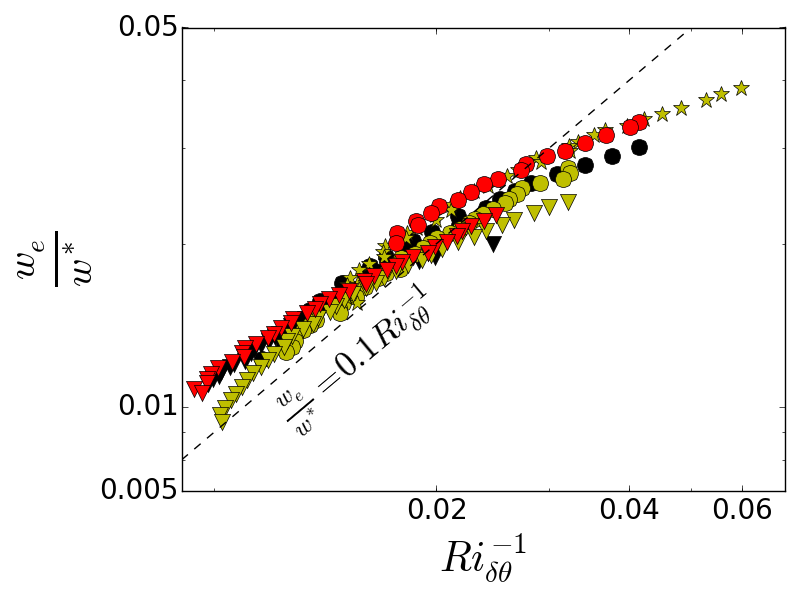
\includegraphics[scale=.3]{figures/scaledweinvri_delta_f_GM.png}}\\
        \subfloat[]{\label{main:b}
                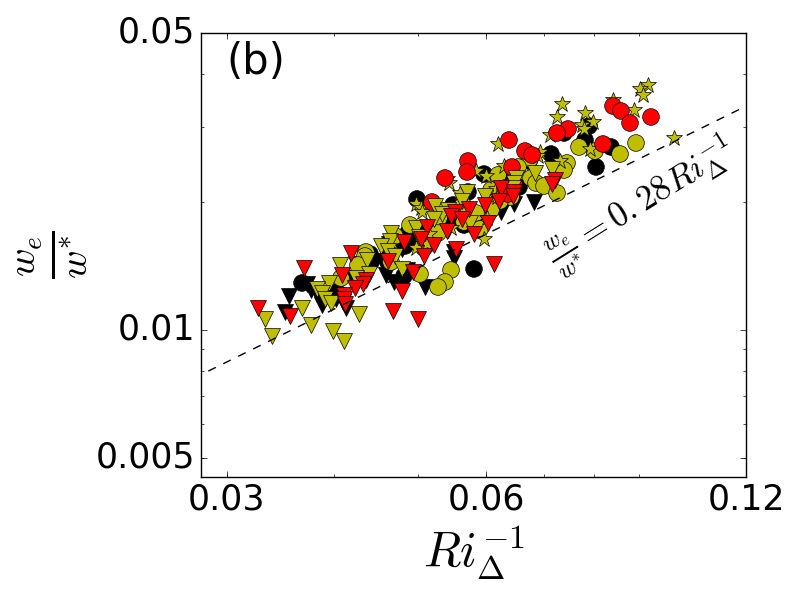
\includegraphics[scale=.3]{figures/scaledweinvri_Delta_f_GM.png}}\\
                     
\end{minipage}             
\begin{minipage}[b]{0.5\linewidth}
        %3b236f get_limits.py, 83b2617 plot_height.py
        \subfloat[]{\label{main:a}
                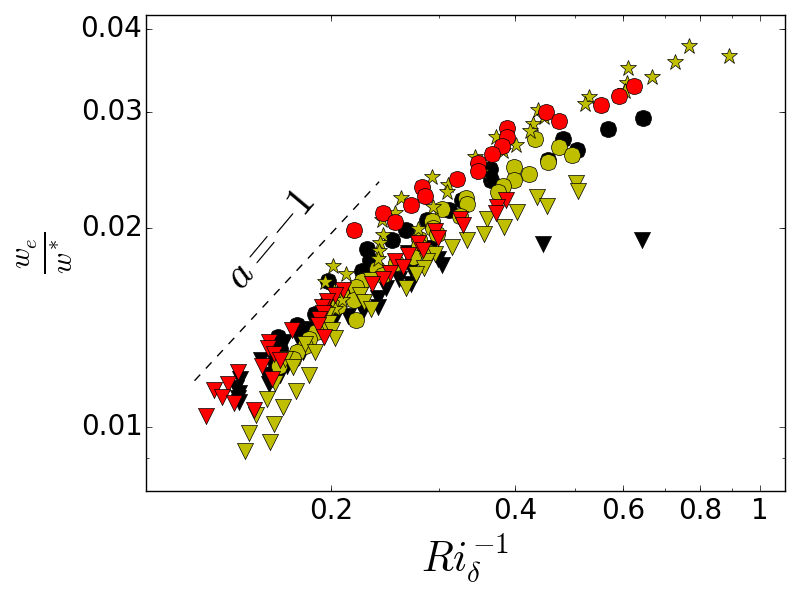
\includegraphics[scale=.3]{figures/scaledweinvri_delta.png}}\\
       % \subfloat[]{\label{main:b}
        %        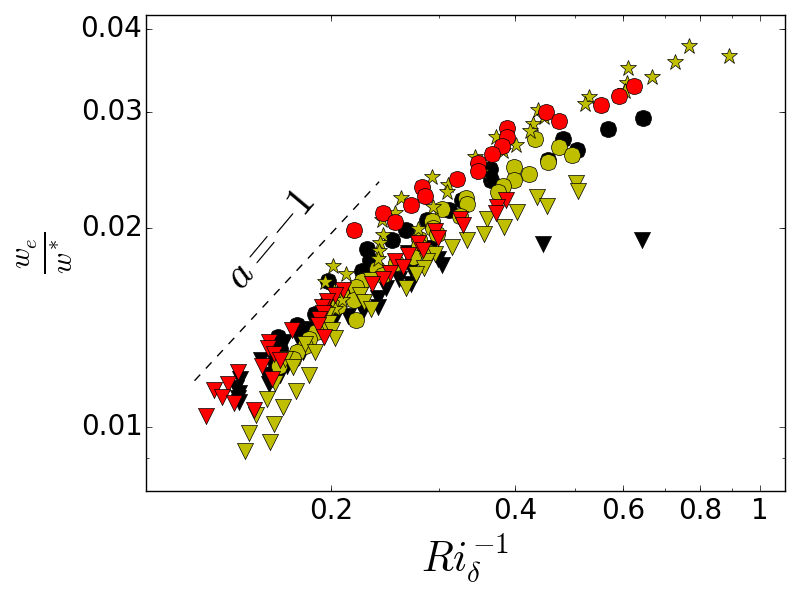
\includegraphics[scale=.3]{figures/scaledweinvri_delta.png}}\\
                     
\end{minipage}             
\quad
\begin{minipage}[b]{0.5\linewidth}
        %\subfloat[]{\label{main:c}          
          %06930 get_limits.py, 0b8ae75 plot_height.py
         %       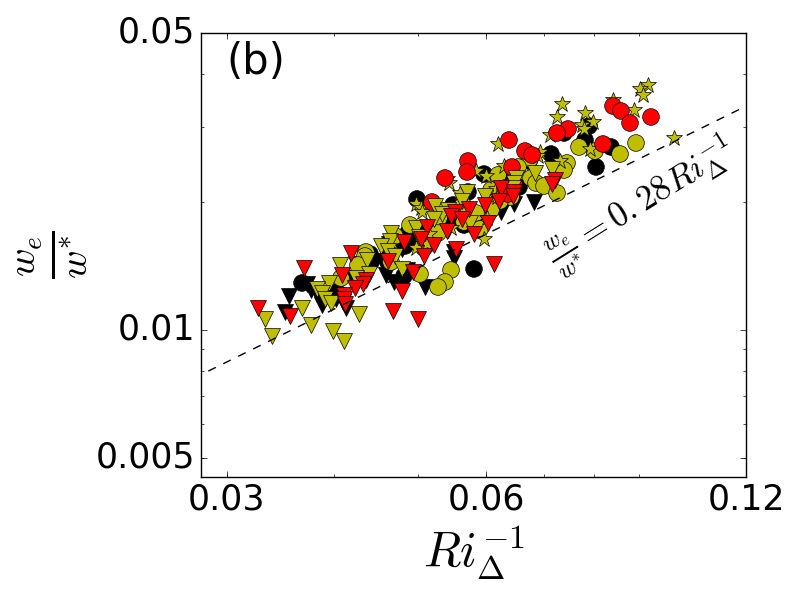
\includegraphics[scale=.3]{figures/scaledweinvri_Delta_f_GM}}\\      
        \subfloat[]{\label{main:d}          
          
                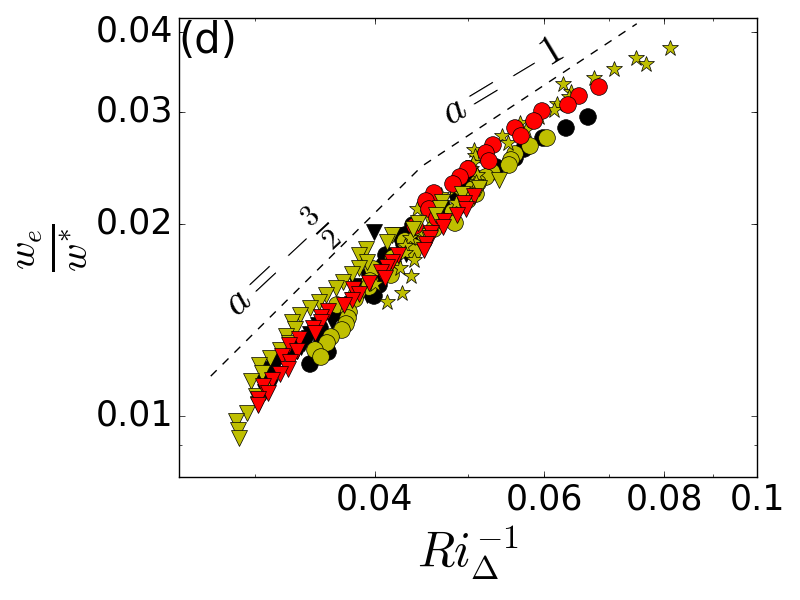
\includegraphics[scale=.3]{figures/scaledweinvri_Delta}
}\\      
       
        \end{minipage}
        \caption{Plots of $\frac{w_{e}}{w_{*}} \propto Ri^{a}$ using height definitions based on the scaled vertical heat flux profile with straight lines predicted by \cite{Garcia14} are in (a) and (b).  (c) and (d) show this relationship when heights are based on the scaled average potential temperature gradient profile. In both sets of plots $\Delta$ represents the temperature jump accross the EZ whereas $\delta$ represents that taken at the CBL top. Legend key:{\color{red} \ding{116}} 150/10 \hspace{3mm}{\color{red} \ding{108}} 150/5 \hspace{2mm} {\color{black} \ding{116}} 100/10 \hspace{2mm} {\color{black} \ding{108}} 100/5 \hspace{2mm} {\color{offyellow} \ding{116}} 60/10 \hspace{2mm} {\color{offyellow} \ding{108}} 60/5 \hspace{2mm} {\color{offyellow} \ding{72}} 60/2.5}
        \label{fig:weinvri}
\end{figure}


\subsubsection{Height definitions based on $\frac{\frac{\partial \overline{\theta}}{\partial z}}{\gamma}$ profile}
In Figure \ref{fig:weinvri} (c) and (d) all heights are based on the $\frac{\frac{\partial \overline{\theta}}{\partial z}}{\gamma}$ profile.  Again, there is a difference in exponent when $\Delta \theta$ is used as compared to when $\delta \theta$ is used.  In Fig. \ref{fig:weinvri} (c) $a=-\frac{3}{2}$ fits at higher $Ri$ (lower $Ri^{-1}$) and $a=-1$ seems to fit at lower $Ri$.  Combined with the apparent change in $b$ for Equation \ref{eq:dhvsri}, we interpret this as an indication of entrainment regime change with increasing $Ri$.\\ 


\section{Conclusions}

\subsection{The gradient method for determining local CBL height, based on the potential temperature profile, is conceptually and practically flawed.  A regression or curve fitting method is better.}

Local $\theta$ profiles vary depending on location.  The top of an active thermal impinging on the free atmosphere (FA) as in Fig. \ref{fig:rssfitshigh} is characterized by a steep gradient comparable to the zero-order jump model representation.  At other locations, for example where a thermal has overturned or recoiled and some entrainment has been initiated as in Fig. \ref{fig:rssfitshigh}, there is a region over which the $\theta$ profile transitions to the upper lapse rate ($\gamma$). That is, there is a local entrainment zone (EZ).  At such locations, there are gradients well into the FA that exceed any within the EZ, as well as an absence of a well-defined local CBL height.  This presents both a practical and conceptual challenge to the gradient method.  Based on hundreds of individual local $\theta$ profiles, determination of the ML height using piecewise linear regression makes more sense visually and is more reliable. 

\subsection{The scaled average vertical potential temperature profile is a valid framework for defining CBL height and EZ boundaries}

The $\overline{\theta}$ profile characterizes the dry, idealized CBL and links bulk models to soundings via an LES.  Both the EZ depth and CBL height based on the average $\frac{\frac{\partial \overline{\theta}}{\partial z}}{\gamma}$ profile showed dependence on $Ri$ as seen in other studies and justified theoretically.  

\subsection{$\gamma$ should be included in any set of scales representing CBL entrainment.}

The magnitude and variance of local ML height, increase with increasing $\overline{w^{'}\theta^{'}}_{s}$, and decrease with increasing $\gamma$.  The same can be said for the vertical velocity fluctuations ($w^{'}$) in the EZ.  However, increased $\gamma$ results in an increase in the positive potential temperature fluctuations ($\theta^{'+}$) at $h$ \citep{NChap14}. The magnitude of ($\theta^{'+}$) at points where $w^{'}$ is negative represents downward moving entrained air and depends on $\gamma$.  Below $h$, in the lower EZ, the average vertical potential temperature gradient ($\frac{\partial \overline{\theta}}{\partial z}$) also depends on $\gamma$. So, the growth of the idealized dry CBL is driven by $(\overline{w^{'}\theta^{'}})_{s}$ and suppressed by stability ($\gamma$). But CBL warming is due, in part, to the entrainment of air from aloft the potential temperature of which in turn depends on $\gamma$.\\

Distributions of scaled local ML heights approach similarity, when $\gamma$ is constant but $(\overline{w^{'}\theta^{'}})_{s}$ is varied.  Curves representing Equation \ref{eq:dhvsri} group according to $\gamma$ when based on the $\frac{\partial \overline{\theta}}{\partial z}$ profile, but collapse once based on $\frac{\frac{\partial \overline{\theta}}{\partial z}}{\gamma}$.  The convective time scale $\tau = \frac{w_{*}}{h}$ and $Ri$ group according to $\gamma$ lending support to \cite{FedConzMir04}'s use of the Brunt-V{\"a}is{\"a}l{\"a} time scale \citep{NChap14}.  It seems that once the effect of the surface heat flux ($\overline{w^{'}\theta^{'}}_{s}$) is accounted for through $h$, $\gamma$ emerges as the dominant parameter in dry, idealized CBL entrainment.\\
 
\subsection{$Ri$ dependence of the scaled EZ depth and entrainment rate changes as $Ri$ increases.}

\cite{Turner86} outlined and theoretically justified two distinct convective boundary layer entrainment regimes wherein the scaled entrainment rates have different $Ri$ dependence. The LES flow visualizations of \cite{Sullivan98} showed large scale engulfment at lower $Ri$.  At higher $Ri$, trapping of smaller volumes of stable air between and at the edges of impinging thermals appeared to be the dominant mechanism. The CBL entrainment zone measurements analyzed in \cite{Traum11} further support the concept of varying entrainment mechanism depending on the strength of the upper lapse rate $\gamma$.  Finally, both \cite{FedConzMir04} and \cite{Garcia14} discuss the varying dependence of the scaled entrainment rate on $Ri$ as the effects of upper stability become more important.  On these grounds the change in exponent in the plots of Eq.s \ref{eq:dhvsri} and \ref{eq:ervsri} in Figures \ref{fig:scaleddeltahinvri} and \ref{fig:weinvri} can be attributed to a change in entrainment regime as $Ri$ increases.   



\begin{acknowledgements}
NSERC CREATE-AAP and NSERC Discovery grants to Douw Steyn and Phil Austin (funding), Compute Canada (computational resources), Python, Matplotlib, Scipi, Cython, Constantine Evans (scikits-bootstrap) 
\end{acknowledgements}


% BibTeX users please use one of
\bibliographystyle{spbasic}      % basic style, author-year citations
%\bibliographystyle{spmpsci}      % mathematics and physical sciences
%\bibliographystyle{spphys}       % APS-like style for physics
\bibliography{nchap_sub}   % name your BibTeX data base




\end{document}
% end of file template.tex


%%% Local Variables:
%%% mode: latex
%%% TeX-master: t
%%% End:
